%%%%%%%%%%%%%%%%%%%%%%%%%% lecture-1
%\begin{frame}
%  \frametitle{lecture-1 主要内容}
%  \tableofcontents[hideallsubsections]
%\end{frame}

\section{课程介绍}

\begin{frame}[shrink]{课程内容}
\begin{itemize}
	%\setlength{\itemsep}{.5cm}
	\item 计算机导论:了解计算机的基本知识;掌握计算机操作基本技能。
	\item 程序设计:掌握结构化程序设计方法, 训练程序逻辑思维能力。会读、会编、会调试C语言程序。
	\item 学习方法:线上、线下相结合。课堂笔记, 认真完成上机练习作业, 鼓励大量编程练习。
	\item 教材
	\begin{itemize}
		\item 大学计算机,龚尚福, 贾澎涛,西安电子科技大学出版社
		\item C程序设计第五版, 谭浩强,清华大学出版社
	\end{itemize}
	%\item 智慧教育平台(使用Chrome浏览器): 
	%\href{https://cvnis.xidian.edu.cn/}{ https://cvnis.xidian.edu.cn/}
	\item 线上参考课程资源链接:
	%\href{run:./online resource.pdf}{online resource.pdf}
	\href{./online resource.pdf}{online resource.pdf} % 可以不使用run
\end{itemize}
\end{frame}

\begin{frame}{线上导论部分学习内容}
\begin{enumerate}
	\setlength{\itemsep}{.8cm}
	\item 计算机历史、现状、发展趋势与前沿技术概述
	\item 计算机体系结构及其编码方式
	\item 计算机组成与软件系统
	\item 计算机应用实践
\end{enumerate}
\end{frame}

\begin{frame}{考核}
\begin{enumerate}
	\setlength{\itemsep}{.5cm}
	\item 平时成绩: 10\%~根据上机练习作业成绩考核。
	\item 导论部分: 20\%~结合线上资源, 自学字处理软件。总结知识点、课堂笔记,撰写课程学习报告。
	\item 期中考试: 30\%~根据机试系统给出的题目编写程序,通过调试得到正确结果并通过\textbf{机试系统提交}。
	\item 期末考试: 40\%~根据机试系统给出的题目编写程序,通过调试得到正确结果并通过\textbf{机试系统提交}。
\end{enumerate}
\end{frame}

\section{导论简介}

\begin{frame}{计算机导论主要内容}
\textbf{总体要求: 了解计算机的基本知识; 掌握计算机操作基本技能。}\\
\begin{itemize}
	\item 计算机系统组成
	\item 计算机工作原理
	\item 操作系统
	\item 字处理: Microsoft Word
	\item 电子表格: Microsoft Excel
	\item 演示文稿: Microsoft PowerPoint
\end{itemize}
\end{frame}

\begin{frame}{计算机工作原理}
\textbf{工作原理: ``存储程序'' + ``程序控制''}
\begin{enumerate}
	\item 以\textbf{二进制}形式表示数据和指令
	\item 将程序存入存储器中,由控制器自动读取并执行
	\item 外部存储器存储的程序和所需数据$\implies$计算机内存$\implies$在程序控制下由CPU周而复始地取出指令、分析指令、执行指令$\implies$操作完成。	
\end{enumerate}
\centering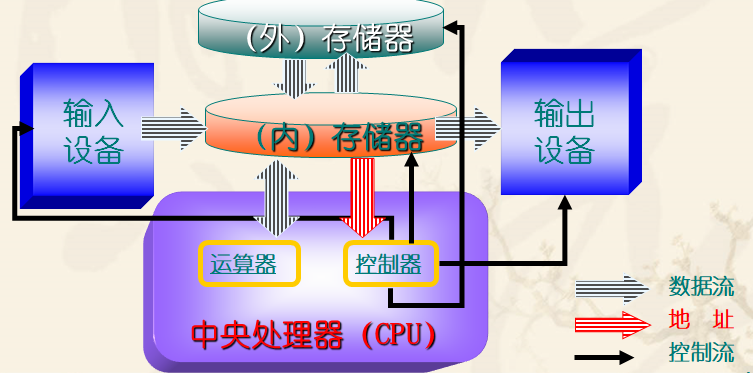
\includegraphics[scale=0.25]{hframe}
\end{frame}

\section{C语言程序设计简介}

\begin{frame}{计算机程序}
\centering

\includegraphics[scale=0.4]{program1}
\end{frame}

\begin{frame}{计算机语言}
\centering
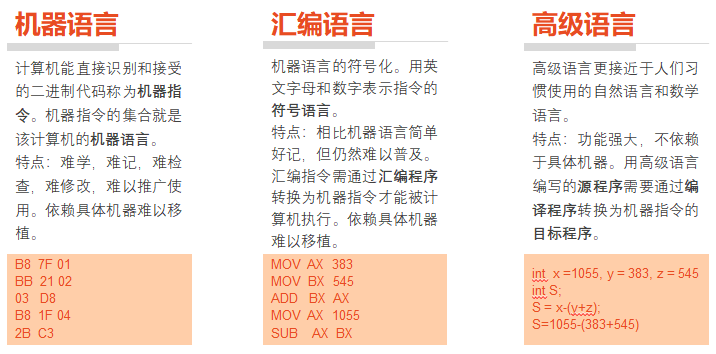
\includegraphics[scale=0.4]{program2}
\end{frame}

\begin{frame}{高级语言的发展}
\centering
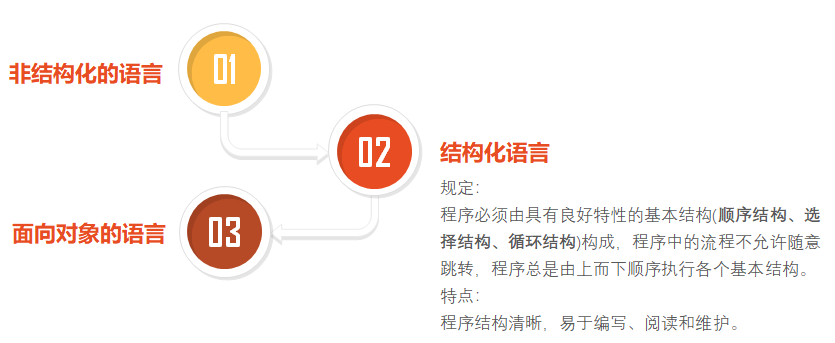
\includegraphics[scale=0.4]{program3}
\end{frame}

\begin{frame}{C语言的特点}
\vspace{-0.5cm}
\begin{enumerate}
	\item 语言简洁、紧凑,使用方便、灵活
    \item 运算符丰富
    \item 数据类型丰富
    \item \textcolor{blue}{C语言是完全模块化和结构化的语言}\\
          具有结构化的控制语句(顺序、选择、循环结构)\\
          用函数作为程序的模块单位,便于实现程序的模块化
    \item \textcolor{blue}{兼具高级语言和低级语言的功能}\\
          允许直接访问物理地址\\
          能进行位(bit)操作\\  
          能实现汇编语言的大部分功能\\
          可以直接对硬件进行操作        
\end{enumerate}
\end{frame}

\begin{frame}{程序设计的任务}
\centering
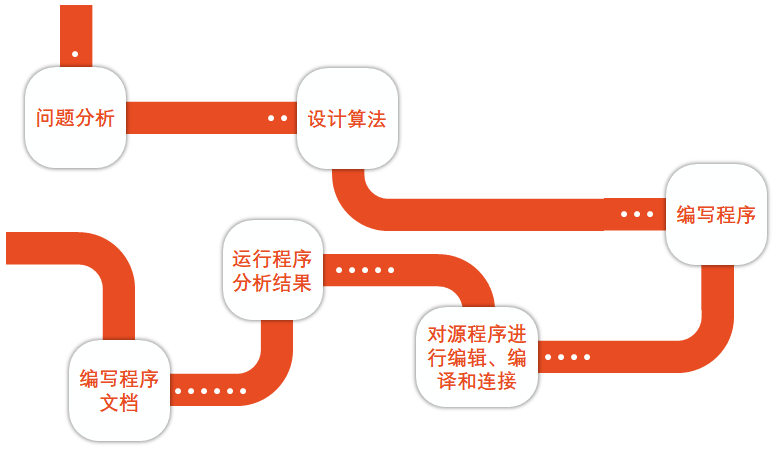
\includegraphics[scale=0.4]{program}
\end{frame}

\begin{frame}[fragile]{第一个C语言程序}
    \begin{lstlisting}
    #include<stdio.h>            // standard input/output编译预处理指令
    int main()                   // 主函数
    {                            // 函数开始标志
       printf("Hello World!");   // printf函数,输出一行信息
       return 0;                 // 函数执行完毕返回函数值0
    }                            // 函数结束标志
    \end{lstlisting}
\end{frame}

\begin{frame}[fragile]{求两个整数之和}
\begin{lstlisting}
#include<stdio.h>         // standard input/output编译预处理指令
int main()                // 主函数
{                         // 函数开始标志
   int a,b,sum;           // 定义a,b,sum为整型变量
   a=123;                 // 对变量a赋值
   b=456;				  // 对变量b赋值
   sum=a+b;               // 计算a+b, 并把结果存放在变量sum中
   printf("sum is %d\n",sum);// printf函数,输出结果
   return 0;                 // 函数执行完毕返回函数值0
}                            // 函数结束标志
\end{lstlisting}
\end{frame}

\begin{frame}[fragile]{求5!的C语言程序。\small{[作业: 请抄写以下各页,并试着分析理解。]}}
\begin{lstlisting}
#include<stdio.h>            // standard input/output编译预处理指令
int main()                   // 主函数
{                            // 函数开始标志
	int i,p;  // p表示被乘数, i表示乘数
	p=1;	  // 对变量p赋值
	i=2;      // 对循环变量i赋值
	while(i<=5) // 循环结构
	{  
		p=p*i;  // =右端p记录本语句执行前的值,左端p记录执行后p的值。
		i++;    // i = i + 1
	}
	printf("%d\n",p);        // printf函数, 输出p的计算结果
	return 0;                // 函数执行完毕返回函数值0
}                            // 函数结束标志
\end{lstlisting}
\end{frame}

\section{开发工具}

\begin{frame}{运行C程序的步骤与方法}
\centering
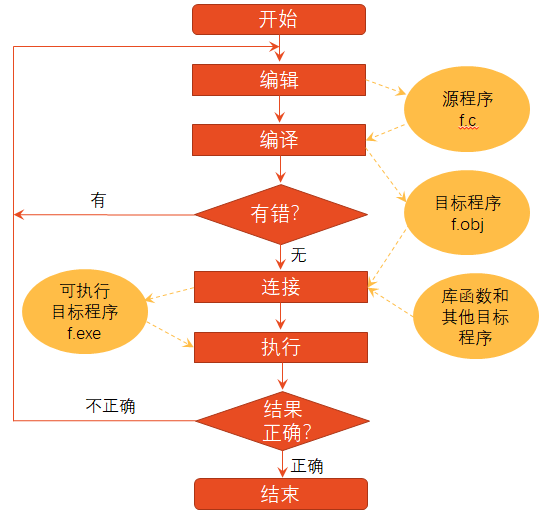
\includegraphics[scale=0.45]{program4}
\end{frame}

\begin{frame}{集成开发环境---编译系统}
\begin{itemize}
\setlength{\itemsep}{.5cm}
\item Bloodshed Dev-C++ 
\item Turbo C
\item Visual C++6.0 
\item Visual Studio(VS2015,VS Community 2019等)
\end{itemize}
\end{frame}

\begin{frame}{Bloodshed Dev-C++集成开发环境}
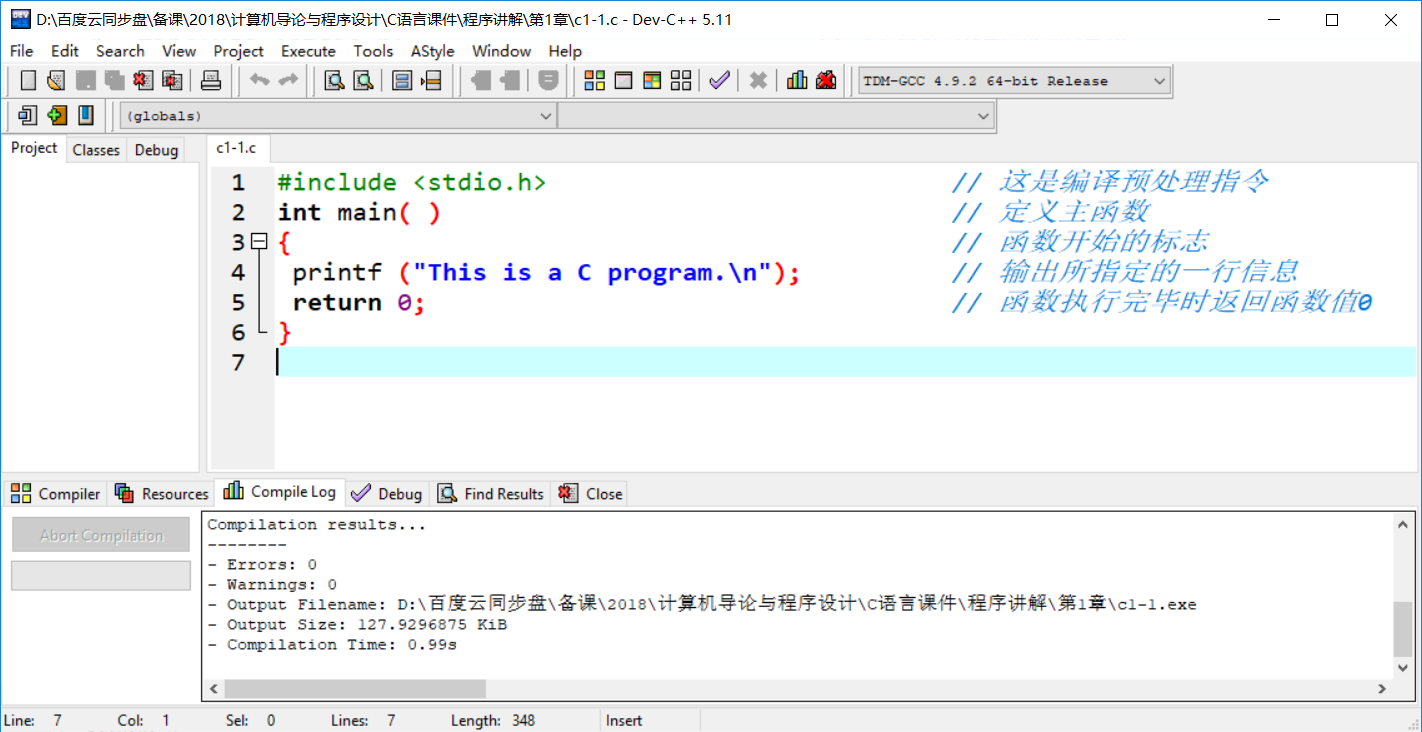
\includegraphics[scale=0.24]{DevCpp}   
\end{frame}

\begin{frame}{Bloodshed Dev-C++集成开发环境}
\vspace{-0.3cm}
\begin{itemize}
\item 选择“文件”菜单,选择“源文件”, 编辑程序。
\item 保存时,保存为 .cpp或 .c文件。
\item 选择“编译和运行”菜单,生成.exe文件,运行程序。  
\end{itemize}
\centering 
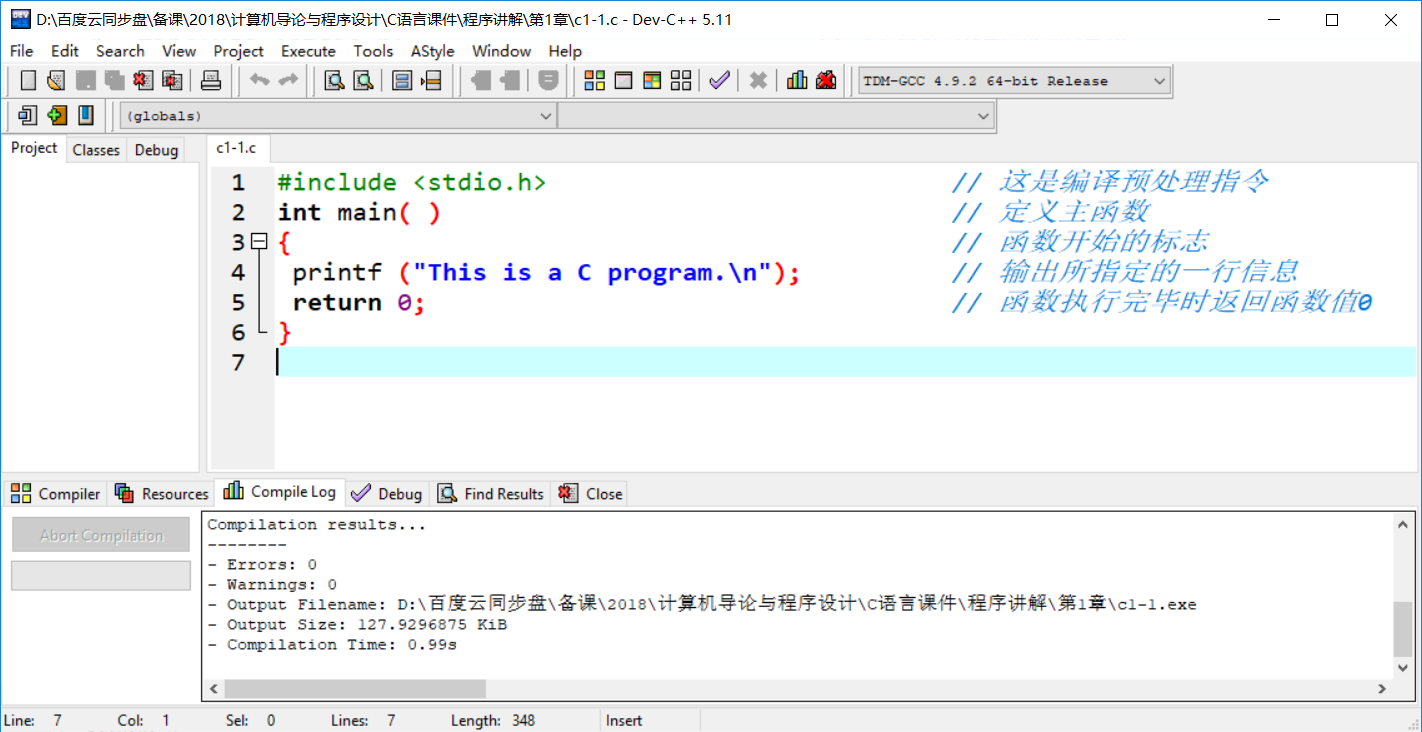
\includegraphics[scale=0.2]{DevCpp}   
\end{frame}
